%% DD-Mamba — Neurocomputing (Elsevier) submission version.
%% Compile: pdflatex -> bibtex -> pdflatex x2 (elsarticle.cls + elsarticle-num.bst).
\documentclass[review,12pt]{elsarticle}

\usepackage[T1]{fontenc}
\usepackage{graphicx}
\usepackage{amsmath,amssymb}
\usepackage{booktabs}
\usepackage{multirow}
\usepackage{url}
\usepackage{tikz}
\usepackage{xcolor}
\usetikzlibrary{positioning,arrows.meta,fit,backgrounds,calc}

% --- shared figure palette (muted, colourblind-friendlier) ---
\definecolor{cNorm}{HTML}{2A9D8F}
\definecolor{cTime}{HTML}{2C6FBB}
\definecolor{cFreq}{HTML}{E07B39}
\definecolor{cFuse}{HTML}{7A5AA6}
\definecolor{cSide}{HTML}{2A9D8F}
\definecolor{cMix}{HTML}{7A5AA6}
\definecolor{cInk}{HTML}{22303C}
\definecolor{cTimeBG}{HTML}{EAF1FB}
\definecolor{cFreqBG}{HTML}{FDF0E6}

\newcommand{\model}{DD-Mamba}
\newcommand{\best}[1]{\textbf{#1}}
\newcommand{\second}[1]{\underline{#1}}

\journal{Neurocomputing}

\begin{document}

\begin{frontmatter}

\title{\model{}: A Forecast-Decomposable State-Space Framework for
Diagnosing When Time, Frequency, and Cross-Variable Components Help
Multivariate Forecasting}

%% TODO (submission): real author list, affiliations, ORCIDs, and the
%% corresponding author. Neurocomputing review is single-anonymized, so
%% author information IS included at submission.
\author[aff1]{First Author\corref{cor1}}
\ead{first.author@example.edu}
\author[aff1]{Second Author}
\cortext[cor1]{Corresponding author.}
\address[aff1]{Department, University, City, Country}

\begin{abstract}
From power grids to road networks, long-term multivariate forecasting must
capture local time-domain dynamics, periodic structure that is compact in
the frequency domain, and cross-channel dependencies whose strength varies
enormously across datasets: the mean absolute inter-channel correlation
spans $0.31$ on ETTh1 to $0.91$ on Solar. Combining time- and
frequency-domain representations, and doing so with state-space backbones,
is by now well explored. We therefore do not claim dual-domain or
time--frequency Mamba modeling as novel; instead we ask \emph{when} each
component actually pays. We present \model{}, a \emph{forecast-decomposable}
state-space framework built for that question: a decomposition-based time
branch and a learned spectral branch each emit a full forecast, combined by
a constrained convex gate, so either branch can be removed and its
contribution measured directly; a DLinear-style backbone with
zero-initialized corrections keeps the initial prediction linear in the
instance-normalized window; and a bidirectional Mamba over variates is a
per-dataset switch guided by measured channel coupling. In a unified
same-pipeline comparison against seven baselines (five shared seeds, so
differences are paired), \model{} has the lowest average MSE on five of six
re-run benchmarks and significantly beats the best in-pipeline baseline on
four under Benjamini--Hochberg correction (Electricity, ETTh2, ETTm2,
ETTh1); it ties on Weather and is beaten by PatchTST on ETTm1. Three further
datasets remain quoted-only pending reruns, so we frame accuracy claims to
the same-pipeline evidence rather than a blanket state-of-the-art assertion.
The framework's further purpose is diagnostic. Across 83
seed-paired comparisons with Benjamini--Hochberg control, all 29
component-placement effects are exploratory (none survive correction at
$n{=}3$), while 9 of 54 branch-removal tests survive: the time branch is
robustly necessary on the ETTm datasets, whereas confirmatory evidence for
the frequency branch is limited to Solar at the 96-step horizon. \model{}
thus offers a reproducible way to diagnose conditional component
effectiveness --- which data characteristics reward which components ---
rather than another universally superior forecaster.
\end{abstract}

\begin{keyword}
Time series forecasting \sep State-space models \sep Mamba \sep
Frequency domain \sep Multivariate analysis
\end{keyword}

\end{frontmatter}

\section{Introduction}

Long-term forecasting of multivariate time series underpins applications
from power-grid load planning to traffic management and weather-dependent
operations. The field has cycled through architectural paradigms at a
remarkable pace: Transformer variants with efficient attention
\cite{informer,autoformer,fedformer}, patch-based attention
\cite{patchtst}, inverted variate-token attention \cite{itransformer},
and, most recently, selective state-space models (SSMs) built on Mamba
\cite{mamba,smamba,msmamba}, which offer linear-time sequence modeling with
input-dependent dynamics.

Combining time- and frequency-domain representations is itself an
established direction: TF4TF \cite{tf4tf} models multi-semantic
time--frequency information for long-term forecasting, and recent work pairs
time--frequency or decomposition-based modeling with Mamba backbones
\cite{decmamba,msmamba}. We therefore do \emph{not} position dual-domain
forecasting or a time--frequency Mamba as our contribution. What remains
under-examined is a different question --- \emph{when} does each such
component actually pay? Existing dual-domain models fuse representations
inside the network, so the time view, the spectral view, normalization, and
cross-variate capacity are entangled and cannot be individually switched
off and measured. Our contribution is a \emph{forecast-decomposable}
framework that makes exactly these choices separable and testable, together
with the seed-paired, multiplicity-controlled evidence of where each one
helps.

\emph{Three empirical gaps} motivate this design. \textbf{Gap~1: deep
models discard strong linear maps.} A per-component linear projection from
the look-back window to the horizon (DLinear \cite{dlinear}) and a tiny
complex-linear interpolation of the low-passed spectrum (FITS \cite{fits})
can be competitive with much larger models on standard benchmarks. Without
such a direct pathway, a deep architecture must learn any linear behavior
implicitly, which may be inefficient on small datasets.
\textbf{Gap~2: the useful inductive bias differs by domain, but is rarely
separable.} Local trends and regime changes are naturally expressed in the
time domain, while multi-scale seasonality is compact in the frequency
domain. Models committed to a single view --- attention or SSMs over time
steps only, or spectral mixing only \cite{frets} --- expose just one; and
even dual-domain models that use both, such as TF4TF \cite{tf4tf}, fuse them
\emph{inside} the network, so neither view is a separately removable
forecast path whose marginal value can be measured.
\textbf{Gap~3: cross-variate capacity can help or hurt.} Cross-variate
mixing is effective on several high-dimensional benchmarks
\cite{itransformer,smamba,crossformer}, but the underlying data property it
exploits --- how strongly channels are actually correlated --- differs by a
factor of three across the standard benchmarks (Table~\ref{tab:datasets}),
and our controlled results show the same module can overfit a weakly
coupled, low-channel dataset. This motivates treating the mixer as an
explicit, data-diagnosable option rather than a universal setting.

We answer these three gaps with \model{} (Fig.~\ref{fig:arch}), mapping
each to one structural remedy: \emph{(i)}~a DLinear-style time backbone with
zero-initialized nonlinear corrections; \emph{(ii)}~parallel time and
frequency forecasts, including an optional dormant FITS-style spectral map,
fused by a convex gate; and \emph{(iii)}~a bidirectional variate mixer
switched on or off per dataset. Paired ablations test these choices below;
only effects whose confidence intervals exclude zero are treated as supported.

Concretely, the time branch combines a DLinear-style pathway
\cite{dlinear} with a zero-initialized nonlinear correction, while the
frequency branch combines learned filtering with an optional zero-initialized
FITS-style spectral pathway \cite{fits}. The resulting model starts as a
linear map of the instance-normalized window (the RLinear-class structure
\cite{rlinear,revin}); a controlled test finds zero initialization
accuracy-neutral. The branch forecasts form a learned convex combination.
Because each branch emits a full forecast, we can remove it and measure the
effect with seed-paired tests, correcting for multiple comparisons with the
Benjamini--Hochberg (BH) procedure. Two patterns emerge. Component-placement
effects --- the variate mixer helping Weather while hurting ETTh1,
normalization helping Weather while hurting Solar --- are visible at the
raw level but, at three seeds, \emph{none} survive BH correction; we
therefore report them as \emph{exploratory} directional evidence, not
confirmed effects. Branch removal is sharper: of 54 branch tests, 9 survive
BH, and they are dominated by the \emph{time} branch (necessary on ETTm1 at
every horizon and on ETTm2, Electricity, and Exchange at $H{=}96$).
Confirmatory support for the \emph{frequency} branch narrows after
correction to a single cell, Solar at $H{=}96$; its raw significance on
ETTm1, Electricity, Exchange, and ETTm2@336 does not survive BH. The
dual-domain benefit is thus real but sharply conditional, and honestly
characterized as exploratory beyond Solar$@$96.

\noindent\textbf{Contributions.} \textbf{(1)}~A \emph{forecast-decomposable}
framework in which the time branch, spectral branch, normalization, and
cross-variate mixer are each an independently removable component, so their
marginal value can be measured directly rather than inferred from an
end-to-end score; \textbf{(2)}~a multiplicity-controlled diagnostic study
--- 83 seed-paired comparisons with Benjamini--Hochberg correction ---
that reports \emph{which} components are confirmed (the time branch on the
ETTm datasets; the frequency branch only on Solar$@$96) and which are
merely exploratory (all component-placement effects at $n{=}3$), rather
than overclaiming from raw $p$-values; \textbf{(3)}~a concrete architecture
realizing the framework: a DLinear-style time backbone with
zero-initialized corrections (making the initial forecast an interpretable
linear map, shown accuracy-neutral) and an optional dormant spectral
pathway; and \textbf{(4)}~a data-characteristic account --- linking
cross-channel PCC and horizon to component value --- that turns the study
into a practical, validation-only component-selection screen.

\noindent\textbf{Organization.} Section~\ref{sec:related} reviews time
series analysis tasks, deep models for temporal and for cross-dimensional
dependencies, and the resulting research gap. Section~\ref{sec:prelim} formalizes
the forecasting problem and reviews the state-space background \model{}
builds on. Section~\ref{sec:method} details the dual-domain architecture,
its zero-initialized corrections, and the switchable variate mixer.
Section~\ref{sec:experiments} reports the main comparison, paired
ablations, and the branch-ablation matrix; Section~\ref{sec:discussion}
distills practical component-selection guidance and threats to validity;
and Section~\ref{sec:conclusion} concludes.

\section{Related Work}
\label{sec:related}

\subsection{Time Series Analysis Tasks}
Deep models now serve the full
spectrum of time series mining tasks --- forecasting, classification,
anomaly detection, and imputation --- often through shared general-purpose
backbones such as TimesNet \cite{timesnet}, whose representations transfer
across tasks. Long-term multivariate \emph{forecasting}, our setting, is
the most benchmark-standardized of these problems: fixed look-back,
multi-horizon evaluation, and shared splits \cite{informer,itransformer}
make it the natural arena for controlled architectural evidence, and
findings about which structures a dataset rewards typically carry over to
the sibling tasks that reuse forecasting backbones.

\subsection{Temporal-Dependency Models}
One line models dependencies along
the time axis only. Transformer variants adapt attention to long sequences
via sparsity, decomposition, and frequency enhancement
\cite{informer,autoformer,fedformer}, patching \cite{patchtst}, or explicit
de-/re-stationarization \cite{nonstationary}. A second family shows that
\emph{linear} maps remain competitive: DLinear/NLinear \cite{dlinear},
RLinear with reversible instance normalization \cite{rlinear,revin}, the
MLP-based TiDE \cite{tide} and TimeMixer \cite{timemixer}, and the
residual-stacked N-BEATS/N-HiTS \cite{nbeats,nhits}, our closest
residual-forecasting precedents. A third works in the spectrum: FreTS
\cite{frets} learns frequency-domain MLPs and FITS \cite{fits} forecasts
with one complex-linear interpolation of the low-passed spectrum. A fourth,
directly adjacent to us, combines \emph{both} time and frequency views:
TF4TF \cite{tf4tf} mines multi-semantic time--frequency information for
long-term forecasting. Such dual-domain models fuse the two views inside
the network, so --- unlike the framework here --- neither view is a
separately removable forecast path.
Decomposition-based designs (STL \cite{stl}, SCINet \cite{scinet}, and the
seasonal-trend-dispersion view of STD \cite{std}) make component structure
explicit; RevIN, used here as a per-dataset switch, normalizes windows
reversibly but neither extracts nor forecasts dispersion, and we claim no
STD-style decomposition.

\subsection{Cross-Dimensional (Spatial--Temporal) Models}
A second line treats the variate dimension as a first-class axis. Crossformer
\cite{crossformer} is the classic Transformer of this type: it embeds the
series into a two-dimensional patch grid and attends over \emph{both} the
temporal and the cross-variate (spatial) dimension. iTransformer
\cite{itransformer} inverts the axes and attends over variate tokens only;
SOFTS \cite{softs} reaches linear-complexity channel interaction through a
centralized core, and ModernTCN \cite{moderntcn} interleaves temporal and
cross-variable convolutions. Selective state-space models bring linear-time
scans to the same axes: Mamba \cite{mamba,mamba2} over time, and S-Mamba
\cite{smamba}, TimeMachine \cite{timemachine}, and FMamba \cite{fmamba}
over variate tokens, with recent variants adding multi-scale processing
(ms-Mamba \cite{msmamba}) and series decomposition (DecMamba
\cite{decmamba}). \model{} sits in this lineage --- causal Mamba over
time, bidirectional Mamba over variates and frequency bins --- but, rather
than proposing yet another fixed Mamba topology, treats the spatial
dimension as a \emph{switchable} module whose value is measured per
dataset.

\subsection{Research Gap}
Dual-domain forecasting \cite{tf4tf}, time--frequency and decomposition
Mamba hybrids \cite{decmamba,msmamba}, and cross-dimensional attention
\cite{crossformer,itransformer} are all, by now, well-populated spaces; a
new model in any of them is unlikely to be a contribution on its own. What
these lines share is a \emph{methodological} limitation rather than an
architectural one. (i)~Representations are fused inside the network, so the
marginal value of the time view, the spectral view, or a decomposition step
is never separately measured. (ii)~Cross-dimensional models such as
Crossformer apply the same spatial--temporal capacity to every dataset,
although channel coupling varies enormously across benchmarks (mean
absolute cross-channel Pearson correlation ranges from $0.31$ on ETTh1 to
$0.91$ on Solar; Table~\ref{tab:datasets}). (iii)~Component-level
comparisons, when reported at all, typically rest on a handful of seeds and
uncorrected $p$-values, so it is unclear which claimed effects would survive
multiplicity control. The gap we target is therefore diagnostic: no prior
work, to our knowledge, pairs a per-component switchboard with controlled,
multiplicity-corrected, seed-paired evidence of \emph{where} --- for which
datasets, correlation regimes, and horizons --- each structure pays.
\model{} is built to answer exactly that question: independently removable
time/frequency forecast paths, a switchable variate mixer, zero-initialized
corrections in the spirit of ReZero \cite{rezero} (an interpretable
initialization convention, shown accuracy-neutral), and a 27-cell
branch-ablation matrix, analyzed under Benjamini--Hochberg control, that
connects data characteristics to component value.

\section{Preliminaries}
\label{sec:prelim}

\subsection{Problem Formulation}
\label{sec:problem}

Given a look-back window $\mathbf{X} \in \mathbb{R}^{L \times C}$ of $L$
steps and $C$ variates, long-term multivariate forecasting predicts the
next $H$ steps $\mathbf{Y} \in \mathbb{R}^{H \times C}$, with $H$ typically
in $\{96,192,336,720\}$. Following RevIN \cite{revin}, we standardize each
window per variate, $\tilde{\mathbf{X}} = (\mathbf{X} - \boldsymbol{\mu}) /
\boldsymbol{\sigma}$, using the window's own per-variate mean
$\boldsymbol{\mu}$ and standard deviation $\boldsymbol{\sigma}$, and
de-normalize the final forecast by the inverse affine map. Instance
normalization is treated as a per-dataset switch rather than a universal
default; Section~\ref{sec:ablation} shows why. A model is a map
$f_\theta:\tilde{\mathbf{X}}\mapsto\mathbf{Y}$ trained to minimize the mean
squared error over the horizon.

\subsection{State Space Models}
\label{sec:ssm-background}

A continuous linear state-space model maps an input signal $u(t)\in\mathbb{R}$
to an output $y(t)\in\mathbb{R}$ through an $N$-dimensional latent state
$\mathbf{h}(t)\in\mathbb{R}^{N}$,
\begin{equation}
\mathbf{h}'(t) = \mathbf{A}\,\mathbf{h}(t) + \mathbf{B}\,u(t), \qquad
y(t) = \mathbf{C}^{\top}\mathbf{h}(t),
\label{eq:cont-ssm}
\end{equation}
with $\mathbf{A}\in\mathbb{R}^{N\times N}$, $\mathbf{B},\mathbf{C}\in\mathbb{R}^{N}$.
To operate on a discrete sequence, the system is discretized with a step
size $\boldsymbol{\Delta}$ under a zero-order hold, which yields the
discrete parameters
\begin{equation}
\bar{\mathbf{A}} = \exp(\boldsymbol{\Delta}\mathbf{A}), \qquad
\bar{\mathbf{B}} = (\boldsymbol{\Delta}\mathbf{A})^{-1}
(\exp(\boldsymbol{\Delta}\mathbf{A}) - \mathbf{I})\,\boldsymbol{\Delta}\mathbf{B}
\;\approx\; \boldsymbol{\Delta}\mathbf{B},
\label{eq:zoh}
\end{equation}
and turns Eq.~\eqref{eq:cont-ssm} into the linear recurrence
$\mathbf{h}_k = \bar{\mathbf{A}}\,\mathbf{h}_{k-1} + \bar{\mathbf{B}}\,u_k$,
$y_k = \mathbf{C}^{\top}\mathbf{h}_k$. Classical structured SSMs keep
$(\bar{\mathbf{A}},\bar{\mathbf{B}},\mathbf{C})$ fixed across the sequence,
so the recurrence is linear time-invariant and can be evaluated as a global
convolution. Mamba \cite{mamba} makes the model \emph{selective}: the
parameters $(\boldsymbol{\Delta}_k,\mathbf{B}_k,\mathbf{C}_k)$ become
functions of the input $u_k$, so the state transition adapts at each step
and the model can selectively remember or forget context. Selectivity
breaks the convolutional form, but a hardware-aware parallel scan keeps the
cost linear in sequence length. \model{} uses this selective recurrence in
two roles --- a causal scan over time and, optionally, a bidirectional scan
over variates --- detailed next.

\section{Method}
\label{sec:method}

\begin{figure}[tb]
\centering
\resizebox{\textwidth}{!}{%
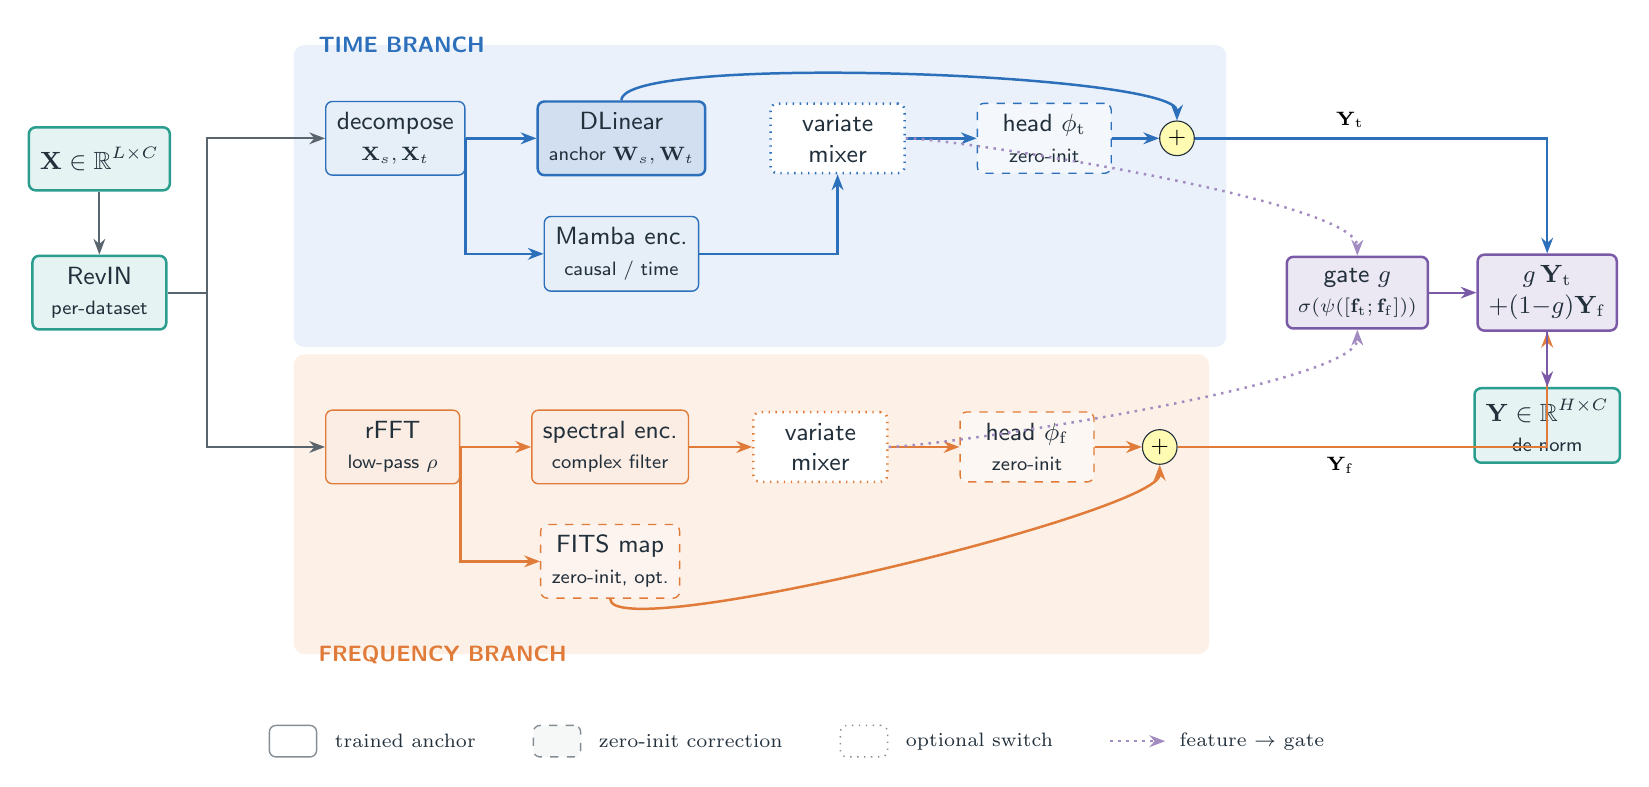
\begin{tikzpicture}[
  font=\sffamily\small,
  >={Stealth[length=2mm]},
  base/.style={draw, rounded corners=2.4pt, align=center, inner sep=4pt,
               minimum height=8mm, minimum width=17mm, line width=0.5pt,
               text=cInk, fill=white},
  norm/.style={base, draw=cNorm, fill=cNorm!12, line width=0.9pt},
  tsolid/.style={base, draw=cTime, fill=cTime!12},
  tanchor/.style={base, draw=cTime, fill=cTime!22, line width=0.9pt},
  tdash/.style={base, draw=cTime, dashed, fill=cTime!5},
  topt/.style={base, draw=cTime, dotted, line width=0.9pt, fill=white},
  fsolid/.style={base, draw=cFreq, fill=cFreq!14},
  fanchor/.style={base, draw=cFreq, dashed, fill=cFreq!8},
  fdash/.style={base, draw=cFreq, dashed, fill=cFreq!6},
  fopt/.style={base, draw=cFreq, dotted, line width=0.9pt, fill=white},
  fuse/.style={base, draw=cFuse, fill=cFuse!14, line width=0.9pt},
  sumc/.style={circle, draw=cInk, fill=yellow!30, inner sep=0pt,
               minimum size=4.4mm, font=\footnotesize},
  flow/.style={->, draw=cInk!75, line width=0.7pt},
  tflow/.style={->, draw=cTime, line width=0.9pt},
  fflow/.style={->, draw=cFreq, line width=0.9pt},
  feat/.style={->, draw=cFuse!70, dotted, line width=0.9pt},
  lane/.style={rounded corners=4pt, inner sep=0pt},
  node distance=6mm and 9mm]

% ---------- input / normalization ----------
\node[norm] (inp) {$\mathbf{X}\in\mathbb{R}^{L\times C}$};
\node[norm, below=8mm of inp] (revin) {RevIN\\{\scriptsize per-dataset}};
\coordinate (split) at ($(revin.east)+(5mm,0)$);

% ---------- time lane (top) ----------
\node[tsolid, above right=10mm and 20mm of revin] (dec) {decompose\\{\scriptsize$\mathbf{X}_s,\mathbf{X}_t$}};
\node[tanchor, right=of dec] (dlin) {DLinear\\{\scriptsize anchor $\mathbf{W}_s,\mathbf{W}_t$}};
\node[tsolid, below=5mm of dlin] (mamba) {Mamba enc.\\{\scriptsize causal / time}};
\node[topt, right=8mm of dlin] (mixT) {variate\\mixer};
\node[tdash, right=of mixT] (headT) {head $\phi_{\mathrm{t}}$\\{\scriptsize zero-init}};
\node[sumc, right=6mm of headT] (sumT) {$+$};

% ---------- freq lane (bottom) ----------
\node[fsolid, below right=10mm and 20mm of revin] (fft) {rFFT\\{\scriptsize low-pass $\rho$}};
\node[fsolid, right=of fft] (spec) {spectral enc.\\{\scriptsize complex filter}};
\node[fanchor, below=5mm of spec] (fits) {FITS map\\{\scriptsize zero-init, opt.}};
\node[fopt, right=8mm of spec] (mixF) {variate\\mixer};
\node[fdash, right=of mixF] (headF) {head $\phi_{\mathrm{f}}$\\{\scriptsize zero-init}};
\node[sumc, right=6mm of headF] (sumF) {$+$};

% ---------- fusion ----------
\node[fuse] (gate) at ($(sumT)!0.5!(sumF)+(24mm,0)$) {gate $g$\\{\scriptsize$\sigma(\psi([\mathbf{f}_{\mathrm t};\mathbf{f}_{\mathrm f}]))$}};
\node[fuse, right=6mm of gate] (comb) {$g\,\mathbf{Y}_{\mathrm t}$\\$+(1{-}g)\mathbf{Y}_{\mathrm f}$};
\node[norm, below=7mm of comb] (out) {$\mathbf{Y}\in\mathbb{R}^{H\times C}$\\{\scriptsize de-norm}};

% ---------- lane bands (behind) ----------
\begin{scope}[on background layer]
  \node[lane, fill=cTimeBG, fit=(dec)(dlin)(mamba)(mixT)(headT)(sumT),
        inner xsep=4mm, inner ysep=7mm] (tband) {};
  \node[lane, fill=cFreqBG, fit=(fft)(spec)(fits)(mixF)(headF)(sumF),
        inner xsep=4mm, inner ysep=7mm] (fband) {};
\end{scope}
\node[anchor=west, text=cTime, font=\sffamily\bfseries\footnotesize]
      at ([xshift=2mm]tband.north west) {TIME BRANCH};
\node[anchor=west, text=cFreq, font=\sffamily\bfseries\footnotesize]
      at ([xshift=2mm]fband.south west) {FREQUENCY BRANCH};

% ---------- edges ----------
\draw[flow] (inp) -- (revin);
\draw[flow] (revin.east) -- (split) |- (dec.west);
\draw[flow] (split) |- (fft.west);
% time internal: anchor (DLinear) skips to the sum; Mamba->mixer->head corrects
\draw[tflow] (dec) -- (dlin);
\draw[tflow] (dec.east) |- (mamba.west);
\draw[tflow] (mamba.east) -| (mixT.south);
\draw[tflow] (mixT) -- (headT);
\draw[tflow] (headT) -- (sumT);
\draw[tflow] (dlin.north) .. controls +(0,6mm) and +(0,6mm) .. (sumT.north);
% freq internal: FITS map skips to the sum; spectral enc->mixer->head corrects
\draw[fflow] (fft) -- (spec);
\draw[fflow] (fft.east) |- (fits.west);
\draw[fflow] (spec) -- (mixF);
\draw[fflow] (mixF) -- (headF);
\draw[fflow] (headF) -- (sumF);
\draw[fflow] (fits.south) .. controls +(0,-6mm) and +(0,-6mm) .. (sumF.south);
% to fusion
\draw[tflow] (sumT.east) -| node[pos=0.22,above,font=\scriptsize]{$\mathbf{Y}_{\mathrm t}$} (comb.north);
\draw[fflow] (sumF.east) -| node[pos=0.22,below,font=\scriptsize]{$\mathbf{Y}_{\mathrm f}$} (comb.south);
\draw[feat] (mixT.east) .. controls +(6mm,0) and +(0,7mm) .. (gate.north);
\draw[feat] (mixF.east) .. controls +(6mm,0) and +(0,-7mm) .. (gate.south);
\draw[flow, draw=cFuse] (gate) -- (comb);
\draw[flow, draw=cFuse] (comb) -- (out);

% ---------- legend ----------
\begin{scope}[shift={($(fband.south west)+(0,-11mm)$)}]
  \node[base, draw=cInk!55, fill=white, minimum width=6mm, minimum height=4mm,
        inner sep=1.5pt] (l1) {};
  \node[right=1mm of l1, font=\scriptsize, text=cInk] (l1t) {trained anchor};
  \node[base, draw=cInk!55, dashed, fill=cInk!4, minimum width=6mm,
        minimum height=4mm, inner sep=1.5pt, right=6mm of l1t] (l2) {};
  \node[right=1mm of l2, font=\scriptsize, text=cInk] (l2t) {zero-init correction};
  \node[base, draw=cInk!55, dotted, minimum width=6mm, minimum height=4mm,
        inner sep=1.5pt, right=6mm of l2t] (l3) {};
  \node[right=1mm of l3, font=\scriptsize, text=cInk] (l3t) {optional switch};
  \draw[feat, right=6mm of l3t] ([xshift=6mm]l3t.east) -- ++(7mm,0)
        node[right=0.5mm,font=\scriptsize,text=cInk]{feature $\to$ gate};
\end{scope}
\end{tikzpicture}}
\caption{\model{} overview. Colour encodes role ---
\textcolor{cNorm}{\textbf{normalization}} (teal),
\textcolor{cTime}{\textbf{time branch}} (blue),
\textcolor{cFreq}{\textbf{frequency branch}} (orange), and
\textcolor{cFuse}{\textbf{convex-gate fusion}} (violet) --- while line style
encodes trainability (legend, bottom): \emph{solid} boxes are trained anchors
(the DLinear backbone, spectral encoder), \emph{dashed} boxes are
zero-initialized corrections (the nonlinear heads $\phi$ and the FITS map),
and \emph{dotted} boxes are per-dataset switches (the variate mixers). Since
every correction starts at zero, the model begins as a scaled linear map of
the instance-normalized window. Dotted violet arrows carry branch features to
the gate, whose convex weight $g$ mixes the two forecast paths
$\mathbf{Y}_{\mathrm{time}}$ and $\mathbf{Y}_{\mathrm{freq}}$.}
\label{fig:arch}
\end{figure}


\subsection{Time Branch: Decomposition, Linear Backbone, Selective Scan}
\label{sec:anchors}

The time branch decomposes $\tilde{\mathbf{X}}$ with a moving average into
trend $\mathbf{X}_t$ and seasonal $\mathbf{X}_s$ components
\cite{autoformer,dlinear} and forecasts with two cooperating paths.

\emph{Linear backbone.} Per-component linear maps project the window
directly to the horizon:
\begin{equation}
\mathbf{Y}_{\mathrm{lin}} = \mathbf{W}_s \mathbf{X}_s +
\mathbf{W}_t \mathbf{X}_t \in \mathbb{R}^{H \times C},
\qquad \mathbf{W}_s, \mathbf{W}_t \in \mathbb{R}^{H \times L},
\end{equation}
i.e., a DLinear-style map \cite{dlinear} (randomly initialized and
trained jointly --- a parameterized pathway, not a fitted DLinear),
shared across variates.

\emph{Selective-scan correction.} The pair $[\mathbf{X}_s; \mathbf{X}_t]$
is embedded per time step and processed channel-independently by a stack
of Mamba layers \cite{mamba} (Fig.~\ref{fig:blocks}a). Instantiating the
selective recurrence of Section~\ref{sec:ssm-background}, the per-step
discrete parameters are
$\bar{\mathbf{A}}_k = \exp(\boldsymbol{\Delta}_k \mathbf{A})$ and
$\bar{\mathbf{B}}_k = \boldsymbol{\Delta}_k \mathbf{B}_k$, and the layer
runs the recurrence
\begin{equation}
\mathbf{h}_k = \bar{\mathbf{A}}_k\,\mathbf{h}_{k-1} +
\bar{\mathbf{B}}_k\, u_k, \qquad
y_k = \mathbf{C}_k^{\top} \mathbf{h}_k + D\, u_k ,
\label{eq:ssm}
\end{equation}
scanned causally over the $L$ steps and applied independently to each of
the $d_{\mathrm{in}}$ feature dimensions: per dimension, the state is
$\mathbf{h}_k \in \mathbb{R}^{N}$, $\mathbf{A} \in \mathbb{R}^{N}$ is
diagonal, the input $u_k$ is scalar, and
$(\boldsymbol{\Delta}_k \in \mathbb{R},\; \mathbf{B}_k, \mathbf{C}_k \in
\mathbb{R}^{N})$ are produced from $u$ by learned linear maps ---
the input-dependent selectivity of \cite{mamba}. The last state, summed
with a whole-window linear embedding $\mathbf{W}_e \tilde{\mathbf{x}}^{(c)}$
(one per variate, as in \cite{smamba}), forms the branch feature
$\mathbf{f}_{\mathrm{time}} \in \mathbb{R}^{C \times d}$. A head
$\phi_{\mathrm{time}}$ maps features to a horizon correction:
\begin{equation}
\mathbf{Y}_{\mathrm{time}} = \mathbf{Y}_{\mathrm{lin}} +
\phi_{\mathrm{time}}(\mathbf{f}_{\mathrm{time}}), \qquad
\phi_{\mathrm{time}} \equiv \mathbf{0} \text{ at init.}
\label{eq:timezero}
\end{equation}
Because $\phi_{\mathrm{time}}$ is zero-initialized, the branch's output at
initialization equals its (randomly initialized) DLinear-style backbone;
the SSM learns only what the linear map cannot express.

\subsection{Frequency Branch: Spectral Filtering and a Dormant Spectral Pathway}
\label{sec:freq}

The frequency branch applies the real FFT along time,
$\mathbf{Z} = \mathrm{rFFT}(\tilde{\mathbf{X}}) \in
\mathbb{C}^{C \times F}$, $F = \lfloor L/2 \rfloor + 1$, optionally
low-passed by zeroing the top fraction $\rho$ of bins.

\emph{Spectral encoder.} A learnable complex linear filter
$\mathbf{W} = \mathbf{W}_r + i\mathbf{W}_i \in \mathbb{C}^{F \times F}$
densely mixes bins, $\mathbf{Z}' = \mathbf{Z}\mathbf{W}^{\top}$ along the
frequency axis (a bidirectional Mamba over the bin sequence is an
input-dependent alternative). The (real, imaginary) parts are projected to
the branch feature $\mathbf{f}_{\mathrm{freq}} \in \mathbb{R}^{C \times d}$
and a head $\phi_{\mathrm{freq}}$ produces the spectral forecast.

\emph{FITS-style spectral pathway (optional, per dataset).} A
complex linear map
$\mathbf{U} \in \mathbb{C}^{F' \times F}$ with
$F' = \lfloor (L{+}H)/2 \rfloor + 1$, applied along the frequency axis
($\mathbf{Z}\mathbf{U}^{\top} \in \mathbb{C}^{C \times F'}$), maps the
(low-passed) window spectrum to that of a length-$(L{+}H)$ series, whose inverse transform's last $H$
samples are the branch's linear spectral forecast:
\begin{equation}
\mathbf{Y}_{\mathrm{freq}} =
\underbrace{\mathrm{irFFT}_{L+H}(\mathbf{Z}\mathbf{U}^{\top})[\,L{:}\,]}_{\text{linear-in-frequency}}
\; + \; \phi_{\mathrm{freq}}(\mathbf{f}_{\mathrm{freq}}),
\qquad \mathbf{U}, \phi_{\mathrm{freq}} \equiv \mathbf{0} \text{ at init.}
\label{eq:fits}
\end{equation}
This pathway uses the frequency interpolation idea of FITS \cite{fits}, but
is not a fitted FITS model: $\mathbf{U}$ is \emph{zero-initialized}, so the frequency branch
is silent at initialization (the length-$L$ and length-$(L{+}H)$ frequency
grids do not align, so no canonical identity init exists, and a random
$\mathbf{U}$ would inject noise during the highest-learning-rate epochs).
With the time head, spectral map, and gate all zero or constant at init, the
end-to-end map in the normalized space is the linear
$g_0\cdot\mathbf{Y}_{\mathrm{lin}}$; composed with RevIN this is the
RLinear-class structure \cite{rlinear,revin} --- linear in the normalized
window, by construction not fitted. The spectral map is enabled per dataset
(Table~\ref{tab:hparams}); where disabled, the frequency branch remains
active through its encoder and forecast head.

\begin{figure}[tb]
\centering
\resizebox{0.92\textwidth}{!}{%
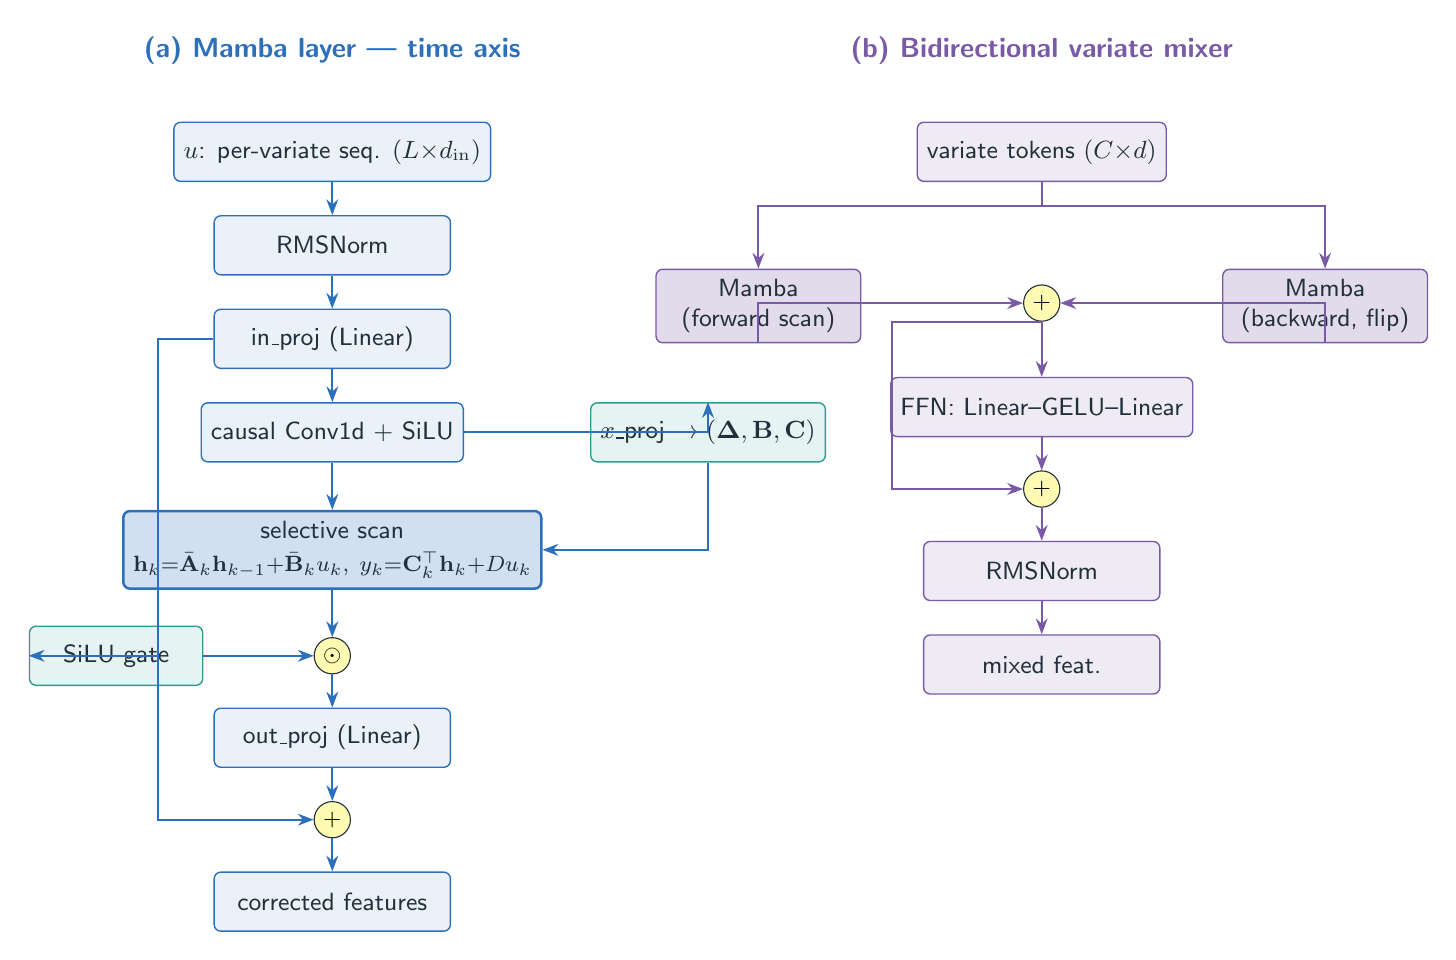
\begin{tikzpicture}[
  font=\sffamily\small,
  >={Stealth[length=2mm]},
  b/.style={draw, rounded corners=2.4pt, align=center, inner sep=3.5pt,
            minimum height=7.5mm, minimum width=30mm, line width=0.5pt,
            text=cInk, fill=white},
  bt/.style={b, draw=cTime, fill=cTime!10},
  scan/.style={b, draw=cTime, fill=cTime!22, line width=0.9pt},
  side/.style={b, draw=cSide, fill=cSide!12, minimum width=22mm},
  bm/.style={b, draw=cMix, fill=cMix!12},
  bms/.style={b, draw=cMix, fill=cMix!22, minimum width=26mm},
  op/.style={circle, draw=cInk, fill=yellow!30, inner sep=0pt,
             minimum size=4.6mm, font=\footnotesize},
  fl/.style={->, draw=cInk!75, line width=0.7pt},
  ft/.style={->, draw=cTime, line width=0.8pt},
  fm/.style={->, draw=cMix, line width=0.8pt},
  node distance=4.2mm]

% ================= (a) Mamba layer =================
\node[bt] (u) {$u$: per-variate seq. $(L{\times}d_{\mathrm{in}})$};
\node[bt, below=of u] (norm) {RMSNorm};
\node[bt, below=of norm] (inp) {in\_proj (Linear)};
\node[bt, below=of inp] (conv) {causal Conv1d $+$ SiLU};
\node[scan, below=6mm of conv] (scan) {selective scan\\[1pt]
  {\footnotesize$\mathbf{h}_k{=}\bar{\mathbf{A}}_k\mathbf{h}_{k-1}{+}\bar{\mathbf{B}}_k u_k,\;
   y_k{=}\mathbf{C}_k^{\top}\mathbf{h}_k{+}Du_k$}};
\node[op, below=6mm of scan] (gate) {$\odot$};
\node[bt, below=of gate] (outp) {out\_proj (Linear)};
\node[op, below=of outp] (res) {$+$};
\node[bt, below=of res] (cf) {corrected features};
% side branches
\node[side, right=16mm of conv] (xproj) {$x$\_proj $\to (\boldsymbol{\Delta},\mathbf{B},\mathbf{C})$};
\node[side, left=14mm of gate] (silu) {SiLU gate};

\draw[ft] (u)--(norm); \draw[ft] (norm)--(inp); \draw[ft] (inp)--(conv);
\draw[ft] (conv)--(scan); \draw[ft] (scan)--(gate);
\draw[ft] (gate)--(outp); \draw[ft] (outp)--(res); \draw[ft] (res)--(cf);
\draw[ft] (conv.east) -| (xproj.north);
\draw[ft] (xproj.south) |- (scan.east);
\draw[ft] (inp.west) -- ++(-7mm,0) |- (silu.west);
\draw[ft] (silu.east) -- (gate.west);
\draw[ft] (inp.west) -- ++(-7mm,0) |- ($(res.west)$);

% ================= (b) Bidirectional variate mixer =================
\node[bm, right=54mm of u] (tok) {variate tokens $(C{\times}d)$};
\node[bms, below left=11mm and 7mm of tok] (fwd) {Mamba\\(forward scan)};
\node[bms, below right=11mm and 7mm of tok] (bwd) {Mamba\\(backward, flip)};
\node[op, below=13mm of tok] (msum) {$+$};
\node[bm, below=7mm of msum] (ffn) {FFN: Linear--GELU--Linear};
\node[op, below=of ffn] (msum2) {$+$};
\node[bm, below=of msum2] (mnorm) {RMSNorm};
\node[bm, below=of mnorm] (mout) {mixed feat.};

\draw[fm] (tok.south) -- ++(0,-3mm) -| (fwd.north);
\draw[fm] (tok.south) -- ++(0,-3mm) -| (bwd.north);
\draw[fm] (fwd.south) |- (msum.west);
\draw[fm] (bwd.south) |- (msum.east);
\draw[fm] (msum) -- (ffn);
\draw[fm] (ffn) -- (msum2);
\draw[fm] (mnorm) -- (mout);
\draw[fm] (msum2) -- (mnorm);
% residual around FFN
\draw[fm] (msum.south) -- ++(-19mm,0) |- (msum2.west);

% ---- panel titles ----
\node[font=\sffamily\bfseries, text=cTime, above=6mm of u]
  {(a) Mamba layer — time axis};
\node[font=\sffamily\bfseries, text=cMix, above=6mm of tok]
  {(b) Bidirectional variate mixer};
\end{tikzpicture}}
\caption{Internal structure of \model{}'s two selective-state-space blocks
(cf.\ the blue boxes in Fig.~\ref{fig:arch}). \textbf{(a)}~The causal Mamba
layer used as the time-axis encoder (Eq.~\eqref{eq:ssm}): an input-dependent
selective scan, gated by a SiLU branch and wrapped in a residual, with
$(\boldsymbol{\Delta},\mathbf{B},\mathbf{C})$ predicted per step from the
input. \textbf{(b)}~The bidirectional mixer used over the \emph{variate}
dimension (Section~\ref{sec:mixer}): forward and backward scans of the $C$
channel tokens summed in one residual stream, then a position-wise
feed-forward block (the S-Mamba design \cite{smamba}).}
\label{fig:blocks}
\end{figure}

\subsection{Cross-Channel Mixing over Variates}
\label{sec:mixer}

Channel independence is a strong baseline \cite{patchtst,dlinear} but
leaves accuracy on the table when variates are coupled
\cite{itransformer,smamba,crossformer}. Inside each branch, before its
head, we optionally run $M$ layers of \emph{bidirectional} Mamba over the
$C$ per-channel features, followed by a position-wise feed-forward block
(Fig.~\ref{fig:blocks}b). Bidirectionality is essential: channel order
carries no causal direction, so each layer sums a forward and a reversed
scan in one residual stream. Whether such mixing \emph{should} pay is a
property of the data: the mean absolute pairwise Pearson correlation (PCC)
between channels on the training split spans $0.31$--$0.35$ on the
weakly coupled ETT family but $0.50$--$0.91$ on Electricity, Traffic, and
Solar (Table~\ref{tab:datasets}). We therefore expose the mixer as a
per-dataset switch --- on for strongly coupled, many-channel benchmarks,
off for weakly coupled, few-channel ones (per-dataset settings in
Section~\ref{sec:setup}) --- and test the decision in both directions in
Section~\ref{sec:ablation}.

\subsection{Forecast-Level Convex Fusion}
\label{sec:fusion}

Each branch emits a forecast and a feature. The model output is a gated
convex combination
\begin{equation}
\mathbf{Y} = g \odot \mathbf{Y}_{\mathrm{time}} + (1 - g) \odot
\mathbf{Y}_{\mathrm{freq}}, \qquad
g = \sigma\!\big(\psi([\mathbf{f}_{\mathrm{time}};
\mathbf{f}_{\mathrm{freq}}])\big) \in (0,1)^{C\times 1},
\label{eq:fusion}
\end{equation}
with $\psi$ applied row-wise (per variate), followed by RevIN
de-normalization. Since $\mathbf{Y}$ lies elementwise between the branch
forecasts, both domains retain an explicit prediction path, and the gate
value reports each branch's convex mixing weight --- a lightweight proxy
for its contribution, not a causal attribution. The constraint is
structural, not behavioral: $g$ is a sigmoid and can saturate near 0 or 1,
so one branch may contribute very little --- by design, as the ablations
show the useful domain is dataset-dependent. $\psi$ is zero-initialized
with its bias set so that training starts gate-open toward the time branch
($g_0 \approx 0.9$; exact value in Section~\ref{sec:setup}): the time branch
is linear at initialization while the frequency branch is silent, and an
even initial mix would halve the initial linear forecast. This is an
initialization convention; empirical gate distributions are not available in
the present study.

\subsection{Training}
We minimize MSE with AdamW under a halving schedule
($\eta_e = \eta_0 \cdot 2^{-(e-1)}$). All runs use 10 epochs with
best-checkpoint early stopping. This schedule was held fixed across our runs
but was not compared with cosine, warm-up, or longer-budget alternatives;
schedule sensitivity therefore remains a potential confound.

\section{Experiments}
\label{sec:experiments}

\subsection{Setup}
\label{sec:setup}

\subsubsection{Datasets and Protocol}
We evaluate on nine standard benchmarks
(Table~\ref{tab:datasets}) under the unified protocol of
\cite{itransformer,smamba}: look-back 96, horizons 96/192/336/720. ETT
uses the canonical 12/4/4-month border split, the others chronological
0.7/0.1/0.2 splits; variates are standardized by training-set statistics;
metrics are MSE and MAE.

\begin{table}[tb]
\centering
\caption{Benchmark datasets, their cross-channel coupling, and where
\model{} places its capacity. $\overline{|r|}$: mean absolute pairwise
Pearson correlation between channels on the training split (--- = raw file
unavailable in our build environment).}
\label{tab:datasets}
\resizebox{\textwidth}{!}{%
\begin{tabular}{@{}lrrlcll@{}}
\toprule
Dataset & Variates & Steps & Granularity & $\overline{|r|}$ & Variate mixer & Params \\
\midrule
ETTh1/ETTh2 & 7 & 17{,}420 & 1 hour & 0.31/0.35 & off & 0.25M \\
ETTm1/ETTm2 & 7 & 69{,}680 & 15 min & 0.31/0.35 & off & 0.24--0.36M \\
Weather & 21 & 52{,}696 & 10 min & --- & $M{=}2$, $d{=}256$ & 5.8M \\
Solar-Energy & 137 & 52{,}560 & 10 min & 0.91 & $M{=}1$, $d{=}128$ & 0.96M \\
Electricity & 321 & 26{,}304 & 1 hour & 0.50 & $M{=}2$, $d{=}512$ & 19.7M \\
Traffic & 862 & 17{,}544 & 1 hour & 0.58 & $M{=}2$, $d{=}512$ & 19.7M \\
Exchange & 8 & 7{,}588 & 1 day & 0.48 & off & 0.09M \\
\bottomrule
\end{tabular}}
\end{table}

\subsubsection{Baselines}
We compare against strong forecasters spanning the linear, patch-attention,
inverted-attention, and state-space families. Crucially, we report the
comparison at \emph{two} levels of rigor. \textbf{(i)~Unified same-pipeline
reruns} (Table~\ref{tab:unified}): DLinear \cite{dlinear}, NLinear
\cite{dlinear}, RLinear \cite{rlinear}, PatchTST \cite{patchtst},
iTransformer \cite{itransformer}, S-Mamba \cite{smamba}, and ms-Mamba
\cite{msmamba} are re-implemented in our codebase and trained through the
\emph{identical} data pipeline, splits, schedule, and evaluation as
\model{}, over five shared seeds --- removing the implementation, split, and
seed confounds that make cross-paper comparison unsafe. These reruns cover
six datasets (ETTh1, ETTh2, ETTm1, ETTm2, Weather, Electricity); because
every model shares seeds, the \model{}-vs-baseline differences are
\emph{paired} and admit proper significance tests. \textbf{(ii)~Quoted
results} (Table~\ref{tab:main}): for the three datasets not yet rerun (Solar,
Traffic, Exchange), and for context on all nine, we additionally show numbers
quoted from \cite{smamba}; these remain \emph{indicative, not confirmatory},
since pipelines and seeds differ across works. The repo-native S-Mamba and
ms-Mamba follow the published designs but are not the authors' code; the
outstanding rerun work is the three quoted datasets and, ideally, the
authors' official implementations (and TF4TF \cite{tf4tf}, which has no public
reference implementation here) through the same adapter.

\subsubsection{Implementation and Reproducibility.}
\label{sec:repro}
All experiments use PyTorch 2.11 (CUDA 13.0) on a single NVIDIA RTX 5090.
Optimization is AdamW (grad clip $5.0$), 10 epochs with the learning rate
halved each epoch, early stopping on validation loss, and mixed precision
with the selective-scan recurrence kept in full precision for numerical
stability of the $L$-step state accumulation. The decomposition kernel is
25; Mamba blocks use expansion 2 and conv width 4 throughout; the fusion
gate's bias is initialized to $2.2$, giving $g_0 = \sigma(2.2) \approx 0.9$
(Section~\ref{sec:fusion}). Table~\ref{tab:hparams} lists all per-dataset settings; configs
and the ablation harness ship with the code. \model{}'s per-horizon results
(Table~\ref{tab:horizons}) are means over \emph{three seeds} (2024--2026);
the maximum per-entry std across the 36 dataset--horizon entries is $0.005$
MSE, typically $0.001$--$0.003$. The unified same-pipeline comparison
(Table~\ref{tab:unified}) uses \emph{five} shared seeds (2024--2028) for
every model, and \model{}'s five-seed averages reproduce its three-seed
numbers to within $0.002$ MSE.
The table records final empirical configurations, not a transferable
capacity-selection rule: no common pre-registered search space or equalized
tuning budget was used across all datasets. Consequently, capacity placement
is reported as an empirical finding, and new datasets require
validation-only selection of these switches.
\subsubsection{Statistical Methodology}
We compare at two levels.
\emph{Within our framework} (ablations), every variant shares seeds with
the reference, so we form the \emph{paired} per-seed difference and report
its mean effect, a two-sided $t$-based $p$-value, and a 95\% CI ($n{=}3$,
$t_{\text{crit}}{=}4.303$). Because we run many such tests, raw $p$-values
overstate significance, so we additionally control the false discovery rate
with the Benjamini--Hochberg (BH) procedure \emph{within each family} --- the
29 component-placement comparisons and the 54 branch-removal comparisons ---
and report the resulting $q$-values (\texttt{scripts/compute\_stats\_correction.py}).
An effect is called \emph{confirmatory} only if it survives BH at $q{<}0.05$;
raw-significant effects that do not survive are reported as
\emph{exploratory}. For the ablations we flag $n{=}3$ as a real limitation of
power; effect sizes with CIs are reported throughout so that readers can
judge magnitude independently of the significance verdict.
\emph{Unified same-pipeline comparison} (Table~\ref{tab:unified}): because
every baseline shares the five seeds with \model{}, we test each
\model{}-vs-baseline difference on the average-over-horizons MSE with a
paired two-sided $t$-test ($n{=}5$, $t_{\text{crit}}{=}2.776$) and
BH-correct across the whole family of comparisons
(\texttt{scripts/analyze\_unified\_baselines.py}); these are the paper's
\emph{confirmatory accuracy} tests.
\emph{Against quoted baselines} (Solar, Traffic, Exchange in
Table~\ref{tab:main}), pairing is impossible, so $0.005$ MSE is
used only as a descriptive tolerance based on the largest standard deviation
among our runs, not as a significance test. Our in-framework DLinear re-run
shows why: through the identical
pipeline on ETTh1 it averages $0.462$/$0.456$ MSE/MAE versus its quoted
$0.456$/$0.452$ --- a $+0.006$ implementation gap, the order of several
margins in Table~\ref{tab:main} --- which is exactly why the same-pipeline
reruns, not the quoted numbers, carry the accuracy claims below.

\begin{table}[tb]
\centering
\caption{Per-dataset hyperparameters. $d$: model width; time enc.:
time-branch encoder (Mamba layers in parentheses); $M$: variate-mixer
layers; $N$: SSM state size; $\rho$: spectral low-pass fraction
(Section~\ref{sec:freq}); spec. map: the \emph{optional} FITS-style pathway of Eq.~\eqref{eq:fits}
--- when ``no'', the frequency branch remains fully active (rFFT, spectral
encoder, forecast head) but carries no explicit linear pathway; IN:
instance normalization (RevIN); do.: dropout; B: batch size; wd: weight
decay. $^{\dagger}$Solar adopts IN~=~no from the ablation finding
(Section~\ref{sec:ablation}); its main results were re-measured under this
configuration across all horizons and seeds.}
\label{tab:hparams}
\scriptsize
\setlength{\tabcolsep}{3.2pt}
\begin{tabular}{@{}lcccccccccc@{}}
\toprule
Dataset & $d$ & time enc. & $M$ & $N$ & $\rho$ & spec. map & IN & lr & B & do./wd \\
\midrule
ETTh1 & 128 & Mamba (1) & 0 & 16 & 0.4 & yes & yes & $5{\cdot}10^{-4}$ & 32 & 0.2/$10^{-4}$ \\
ETTh2 & 128 & Mamba (1) & 0 & 16 & 0.3 & yes & yes & $5{\cdot}10^{-4}$ & 32 & 0.3/$5{\cdot}10^{-4}$ \\
ETTm1 & 128 & Mamba (2) & 0 & 16 & 0 & no & yes & $10^{-4}$ & 32 & 0.1/$10^{-4}$ \\
ETTm2 & 128 & Mamba (1) & 0 & 16 & 0.2 & no & yes & $10^{-4}$ & 32 & 0.2/$2{\cdot}10^{-4}$ \\
Weather & 256 & Mamba (2) & 2 & 16 & 0 & yes & yes & $2{\cdot}10^{-4}$ & 32 & 0.1/$10^{-4}$ \\
Solar & 128 & Mamba (2) & 1 & 16 & 0 & no & no$^{\dagger}$ & $5{\cdot}10^{-4}$ & 16 & 0.1/$10^{-4}$ \\
Electricity & 512 & MLP & 2 & 32 & 0 & no & yes & $5{\cdot}10^{-4}$ & 16 & 0.1/$10^{-4}$ \\
Traffic & 512 & MLP & 2 & 32 & 0 & no & yes & $10^{-3}$ & 16 & 0.1/$10^{-4}$ \\
Exchange & 64 & Mamba (1) & 0 & 8 & 0.5 & no & yes & $10^{-4}$ & 32 & 0.3/$5{\cdot}10^{-4}$ \\
\bottomrule
\end{tabular}
\end{table}

\subsection{Main Results}

\begin{table}[tb]
\centering
\caption{\emph{Quoted-baseline} context (all nine datasets): long-term
forecasting averaged over horizons $H \in \{96,192,336,720\}$, look-back
$L{=}96$ (MSE/MAE; lower is better). \model{} entries are means over three
seeds (Table~\ref{tab:horizons} reports per-horizon std). Baselines
\emph{quoted from} \cite{smamba} --- \emph{indicative, not confirmatory}
(different pipelines/seeds). The confirmatory, same-pipeline comparison for
six of these datasets is Table~\ref{tab:unified}; here the quoted numbers
mainly cover Solar, Traffic, and Exchange, which are not yet rerun.
\textbf{Bold} marks the best result \emph{and} every result within the
descriptive tolerance ($<0.005$, Section~\ref{sec:repro}) of it;
\underline{underline} marks the next-best result.}
\label{tab:main}
\scriptsize
\setlength{\tabcolsep}{2.6pt}
\begin{tabular}{@{}lcccccc@{}}
\toprule
Dataset & \model{} (ours) & S-Mamba & iTransformer & PatchTST & DLinear & TimesNet \\
\midrule
ETTh1 & \best{0.439}/\best{0.434} & 0.455/0.450 & \second{0.454}/\second{0.447} & 0.469/0.454 & 0.456/0.452 & 0.458/0.450 \\
ETTh2 & \best{0.374}/\best{0.401} & \second{0.381}/\best{0.405} & 0.383/\second{0.407} & 0.387/\second{0.407} & 0.559/0.515 & 0.414/0.427 \\
ETTm1 & \best{0.386}/\best{0.398} & \second{0.398}/\second{0.405} & 0.407/0.410 & \best{0.387}/\best{0.400} & 0.403/0.407 & 0.400/0.406 \\
ETTm2 & \best{0.280}/\best{0.325} & \second{0.288}/\second{0.332} & \second{0.288}/\second{0.332} & \best{0.281}/\best{0.326} & 0.350/0.401 & 0.291/0.333 \\
Weather & \best{0.248}/\best{0.276} & \best{0.251}/\best{0.276} & \second{0.258}/\best{0.278} & 0.259/\second{0.281} & 0.265/0.317 & 0.259/0.287 \\
Electricity & \best{0.168}/\best{0.263} & \best{0.170}/\best{0.265} & \second{0.178}/\second{0.270} & 0.205/0.290 & 0.212/0.300 & 0.192/0.295 \\
Traffic & 0.438/\second{0.281} & \best{0.414}/\best{0.276} & \second{0.428}/0.282 & 0.481/0.304 & 0.625/0.383 & 0.620/0.336 \\
Exchange & 0.363/\best{0.405} & 0.367/\second{0.408} & \second{0.360}/\best{0.403} & 0.367/\best{0.404} & \best{0.354}/0.414 & 0.416/0.443 \\
Solar & \best{0.199}/\best{0.260} & 0.240/\second{0.273} & \second{0.233}/\best{0.262} & 0.270/0.307 & 0.330/0.401 & 0.301/0.319 \\
\bottomrule
\end{tabular}
\end{table}

\begin{table}[tb]
\centering
\caption{\model{} per-horizon results (mean $\pm$ std over three
seeds), look-back $L{=}96$.}
\label{tab:horizons}
\scriptsize
\setlength{\tabcolsep}{3.0pt}
\begin{tabular}{@{}llccccc@{}}
\toprule
Dataset & & $H{=}96$ & $H{=}192$ & $H{=}336$ & $H{=}720$ & Avg \\
\midrule
ETTh1 & MSE & $0.380{\scriptstyle\pm.001}$ & $0.431{\scriptstyle\pm.002}$ & $0.474{\scriptstyle\pm.004}$ & $0.470{\scriptstyle\pm.003}$ & 0.439 \\
 & MAE & $0.396{\scriptstyle\pm.001}$ & $0.424{\scriptstyle\pm.001}$ & $0.447{\scriptstyle\pm.003}$ & $0.468{\scriptstyle\pm.001}$ & 0.434 \\
ETTh2 & MSE & $0.293{\scriptstyle\pm.001}$ & $0.368{\scriptstyle\pm.003}$ & $0.414{\scriptstyle\pm.001}$ & $0.421{\scriptstyle\pm.001}$ & 0.374 \\
 & MAE & $0.344{\scriptstyle\pm.002}$ & $0.391{\scriptstyle\pm.000}$ & $0.426{\scriptstyle\pm.000}$ & $0.441{\scriptstyle\pm.001}$ & 0.401 \\
ETTm1 & MSE & $0.320{\scriptstyle\pm.001}$ & $0.366{\scriptstyle\pm.002}$ & $0.398{\scriptstyle\pm.001}$ & $0.462{\scriptstyle\pm.001}$ & 0.386 \\
 & MAE & $0.359{\scriptstyle\pm.001}$ & $0.384{\scriptstyle\pm.001}$ & $0.406{\scriptstyle\pm.001}$ & $0.443{\scriptstyle\pm.001}$ & 0.398 \\
ETTm2 & MSE & $0.177{\scriptstyle\pm.000}$ & $0.242{\scriptstyle\pm.002}$ & $0.302{\scriptstyle\pm.000}$ & $0.401{\scriptstyle\pm.003}$ & 0.280 \\
 & MAE & $0.260{\scriptstyle\pm.001}$ & $0.303{\scriptstyle\pm.001}$ & $0.340{\scriptstyle\pm.000}$ & $0.398{\scriptstyle\pm.002}$ & 0.325 \\
Weather & MSE & $0.162{\scriptstyle\pm.000}$ & $0.212{\scriptstyle\pm.000}$ & $0.269{\scriptstyle\pm.001}$ & $0.352{\scriptstyle\pm.003}$ & 0.248 \\
 & MAE & $0.207{\scriptstyle\pm.001}$ & $0.255{\scriptstyle\pm.000}$ & $0.295{\scriptstyle\pm.002}$ & $0.349{\scriptstyle\pm.002}$ & 0.276 \\
Electricity & MSE & $0.140{\scriptstyle\pm.000}$ & $0.157{\scriptstyle\pm.001}$ & $0.174{\scriptstyle\pm.001}$ & $0.200{\scriptstyle\pm.004}$ & 0.168 \\
 & MAE & $0.235{\scriptstyle\pm.000}$ & $0.252{\scriptstyle\pm.001}$ & $0.271{\scriptstyle\pm.001}$ & $0.296{\scriptstyle\pm.004}$ & 0.263 \\
Traffic & MSE & $0.402{\scriptstyle\pm.002}$ & $0.424{\scriptstyle\pm.001}$ & $0.441{\scriptstyle\pm.001}$ & $0.485{\scriptstyle\pm.003}$ & 0.438 \\
 & MAE & $0.266{\scriptstyle\pm.001}$ & $0.275{\scriptstyle\pm.001}$ & $0.283{\scriptstyle\pm.000}$ & $0.301{\scriptstyle\pm.000}$ & 0.281 \\
Exchange & MSE & $0.086{\scriptstyle\pm.000}$ & $0.179{\scriptstyle\pm.001}$ & $0.330{\scriptstyle\pm.002}$ & $0.857{\scriptstyle\pm.001}$ & 0.363 \\
 & MAE & $0.205{\scriptstyle\pm.000}$ & $0.301{\scriptstyle\pm.000}$ & $0.416{\scriptstyle\pm.002}$ & $0.699{\scriptstyle\pm.000}$ & 0.405 \\
Solar & MSE & $0.180{\scriptstyle\pm.004}$ & $0.195{\scriptstyle\pm.005}$ & $0.207{\scriptstyle\pm.001}$ & $0.212{\scriptstyle\pm.005}$ & 0.199 \\
 & MAE & $0.237{\scriptstyle\pm.003}$ & $0.259{\scriptstyle\pm.003}$ & $0.270{\scriptstyle\pm.001}$ & $0.274{\scriptstyle\pm.005}$ & 0.260 \\
\bottomrule
\end{tabular}
\end{table}

\begin{table*}[tb]
\centering
\caption{\emph{Unified same-pipeline} comparison (average MSE/MAE over
$H\in\{96,192,336,720\}$, look-back $L{=}96$; \textbf{five shared seeds};
lower is better). Every baseline is re-implemented and trained through the
\emph{identical} pipeline, splits, schedule, and evaluation as \model{}, so
differences are \emph{paired}. \best{Bold} marks the lowest per-dataset
mean. $^{*}$\,\model{} beats the best competing baseline at
Benjamini--Hochberg $q{<}0.05$ (paired $t$-test, $n{=}5$;
\texttt{analyze\_unified\_baselines.py}). \model{} has the lowest mean on
five of six datasets and the margin is confirmatory on four
(Electricity, ETTh2, ETTm2, ETTh1); Weather is a statistical tie
($q{=}0.23$) and PatchTST is confirmed better on ETTm1.}
\label{tab:unified}
\scriptsize
\setlength{\tabcolsep}{4pt}
\resizebox{\textwidth}{!}{%
\begin{tabular}{@{}lcccccc@{}}
\toprule
Model & ETTh1 & ETTh2 & ETTm1 & ETTm2 & Weather & Electricity \\
\midrule
\model{} & \best{0.439}/\best{0.434}$^{*}$ & \best{0.376}/\best{0.401}$^{*}$ & 0.387/0.398 & \best{0.280}/\best{0.325}$^{*}$ & \best{0.248}/\best{0.276} & \best{0.168}/\best{0.263}$^{*}$ \\
DLinear & 0.462/0.456 & 0.545/0.509 & 0.410/0.412 & 0.359/0.407 & 0.267/0.318 & 0.211/0.299 \\
NLinear & 0.464/0.450 & 0.390/0.412 & 0.429/0.419 & 0.294/0.337 & 0.279/0.296 & 0.220/0.299 \\
RLinear & 0.457/0.443 & 0.391/0.411 & 0.424/0.413 & 0.293/0.336 & 0.273/0.292 & 0.217/0.295 \\
PatchTST & 0.456/0.449 & 0.385/0.408 & \best{0.381}/\best{0.396} & 0.284/0.331 & 0.249/0.275 & 0.189/0.276 \\
iTransformer & 0.444/0.442 & 0.383/0.407 & 0.407/0.409 & 0.292/0.335 & 0.265/0.285 & 0.195/0.282 \\
S-Mamba & 0.463/0.458 & 0.394/0.410 & 0.397/0.406 & 0.297/0.335 & 0.251/0.278 & 0.183/0.275 \\
ms-Mamba & 0.459/0.451 & 0.409/0.420 & 0.393/0.403 & 0.288/0.333 & 0.257/0.281 & 0.187/0.277 \\
\bottomrule
\end{tabular}}
\end{table*}

Table~\ref{tab:unified} is the paper's primary accuracy evidence, because it
removes the implementation, split, and seed confounds of cross-paper
comparison. Under this same-pipeline, five-seed protocol \model{} has the
lowest average MSE on five of the six re-run datasets, and the paired,
BH-corrected test confirms the margin on \textbf{four}: Electricity
($0.168$ vs.\ S-Mamba's $0.183$; $q\!\ll\!0.01$), ETTh2 ($0.376$ vs.\
iTransformer's $0.383$; $q{=}0.001$), ETTm2 ($0.280$ vs.\ PatchTST's
$0.284$; $q{=}0.015$), and ETTh1 ($0.439$ vs.\ iTransformer's $0.444$;
$q{=}0.021$). Weather is a statistical \emph{tie} --- \model{} is numerically
best ($0.248$ vs.\ PatchTST's $0.249$) but the difference does not survive
correction ($q{=}0.23$). ETTm1 is an honest \emph{loss}: PatchTST is lower
($0.381$ vs.\ $0.387$) and the gap is confirmed ($q{<}0.001$), consistent
with the branch matrix, where ETTm1 is carried by the time branch and its
patch-attention competitor is strong. \model{}'s size is
dataset-dependent: on the low-channel ETT and Exchange datasets it uses only
$\approx\,0.1$--$0.25$M parameters (an order of magnitude fewer than the
variate-attention baselines), whereas on high-channel data the variate mixer
dominates the count and the model is larger (Table~\ref{tab:efficiency});
that mixer cost is itself reducible, as the complexity analysis below notes.
Notably, the confirmatory picture \emph{differs}
from the earlier quoted table (Table~\ref{tab:main}): the clearest
same-pipeline wins are Electricity and ETTh2 rather than the quoted
Solar/ETTh1 headline, and the quoted ETTm1 ``tie'' with PatchTST becomes a
measured loss --- a direct illustration of why quoted comparison is unsafe.

For the three datasets not yet rerun (Table~\ref{tab:main}, quoted, so
\emph{indicative only}), \model{}'s largest apparent margin is Solar ($0.199$
vs.\ iTransformer's $0.233$, with the normalization-free configuration of
Section~\ref{sec:ablation}); it trails DLinear on Exchange (by $0.009$) and
S-Mamba on Traffic (by $0.024$), which we \emph{hypothesize} reflects the
weekly cycle exceeding the look-back. Extending the unified reruns to these
three is the remaining accuracy experiment.

\subsection{Component Ablations}
\label{sec:ablation}

Our ablation harness flips exactly one switch of a dataset's full
configuration, holding split, schedule, seeds, and every other
hyperparameter fixed. We report its complete output on three datasets under
their \emph{final released configurations}, three seeds each at $H{=}96$:
ETTh1 and Solar (Table~\ref{tab:ablation}) and Weather
(Table~\ref{tab:ablation_weather}), with the paired methodology of
Section~\ref{sec:repro}. Two consistency checks pass: the Solar ``full'' row
reproduces the main-table Solar $H{=}96$ entry
($0.180{\scriptstyle\pm.004}$), and its w/o-instance-norm variant coincides
with the full (RevIN-off) configuration, so that cell is omitted.

\begin{table}[tb]
\centering
\caption{Component ablations on ETTh1 and Solar-Energy ($H{=}96$, three
seeds, final configurations): paired per-seed $\Delta$MSE to the full
model with $t$-based 95\% CIs; $^{*}$\,CI excludes zero. The spectral map
is enabled on ETTh1 (hence \emph{removed}) and disabled on Solar (hence
\emph{added}); the variate mixer is off on ETTh1 (\emph{added}) and on
for Solar (\emph{removed}).}
\label{tab:ablation}
\scriptsize
\setlength{\tabcolsep}{3pt}
\begin{tabular}{@{}lcc@{}}
\toprule
Variant & ETTh1: $\Delta$ [95\% CI] & Solar: $\Delta$ [95\% CI] \\
\midrule
full (reference MSE) & $0.3802{\scriptstyle\pm.001}$ & $0.1802{\scriptstyle\pm.004}$ \\
\;\;time branch only (freq removed) & $+0.0034$ $[-0.009,+0.016]$ & $+0.0114$ $[+0.001,+0.021]$$^{*}$ \\
\;\;freq branch only (time removed) & $-0.0007$ $[-0.004,+0.003]$ & $+0.0051$ $[-0.013,+0.023]$ \\
\;\;sum fusion & $-0.0026$ $[-0.007,+0.002]$ & $+0.0066$ $[-0.005,+0.018]$ \\
\;\;w/o instance norm & $+0.0061$ $[-0.001,+0.013]$ & --- \\
\;\;w/o linear backbone & $-0.0031$ $[-0.009,+0.003]$ & $+0.0081$ $[-0.019,+0.035]$ \\
\;\;random init (vs.\ zero-init) & $-0.0012$ $[-0.005,+0.002]$ & $-0.0046$ $[-0.022,+0.013]$ \\
\;\;spectral map removed / added & $+0.0042$ $[-0.018,+0.026]$ & $+0.0088$ $[-0.002,+0.019]$ \\
\;\;variate mixer added / removed & $+0.0077$ $[+0.004,+0.012]$$^{*}$ & $+0.0119$ $[-0.010,+0.034]$ \\
\;\;Mamba$\rightarrow$MLP over time & $-0.0022$ $[-0.007,+0.003]$ & $+0.0089$ $[-0.002,+0.020]$ \\
\;\;freq Mamba encoder & $-0.0024$ $[-0.011,+0.006]$ & $-0.0117$ $[-0.044,+0.020]$ \\
\bottomrule
\end{tabular}
\end{table}

\paragraph{Component-placement effects are directional but exploratory.} A
two-sided pattern spans datasets at the raw level: adding the variate mixer
on ETTh1 \emph{hurts} (by $+0.0077$ MSE, raw $p{=}0.014$) while removing it
on Weather also hurts (by $+0.0104$, raw $p{=}0.022$); normalization shows the
same shape (removing it hurts Weather $+0.0161$, raw $p{=}0.023$, while
disabling it on Solar improved the re-measured main results from $0.228$ to
$0.199$). We emphasize, however, that across the 29 component-placement
comparisons \emph{none} survives Benjamini--Hochberg correction (the five
raw-significant effects have $q\ge 0.11$): at three seeds these are
\emph{exploratory, directional} findings, not confirmed effects, and we
report them as such. The consistency of the \emph{direction} (component
value is dataset-dependent, in both directions) is what motivates
per-dataset switches; confirming any individual effect requires more seeds.
Zero initialization is a \emph{null} result --- no significant difference on
either dataset ($-0.0012$ ETTh1, $-0.0046$ Solar; CIs include zero) --- so
we make no accuracy claim for it, only the interpretable linear start
(Section~\ref{sec:anchors}). The DLinear backbone and the learned gate versus
averaging are within CIs everywhere; on Weather
(Table~\ref{tab:ablation_weather}) three components have unadjusted paired
CIs excluding zero (normalization, the variate mixer, and the temporal Mamba,
$+0.0027$, positive on all seeds). The recurring pattern --- component value
is dataset-dependent, in \emph{both} directions --- is the argument for
per-dataset switches over universal defaults, and it does not depend on any
single dataset.

\paragraph{Branch matrix: where each domain matters.} Because a single
Solar cell cannot carry a dual-domain conclusion, we ran the full
branch-ablation matrix --- full / time-only / freq-only under paired seeds
on all nine datasets at $H{=}96$ and across all four horizons on the six
ETT/Weather/Solar datasets, 27 cells in total
(Table~\ref{tab:branchmatrix}). Every full-model mean reproduces the
corresponding main-table entry, and the Solar $H{=}96$ cell replicates the
earlier ablation ($+0.0126$ vs.\ $+0.0114$, overlapping CIs). The 27 cells
yield 54 branch-removal tests; we report both raw significance (CI excludes
zero, marked $^{*}$ in Table~\ref{tab:branchmatrix}) and BH-corrected
$q$-values, and treat only the latter as confirmatory.

\emph{Frequency branch.} At the raw level, removing it is significant in 5
cells, concentrated at the shortest horizon: Solar ($+0.0126$), ETTm1
($+0.0073$), Electricity ($+0.0019$), and Exchange ($+0.0015$) at $H{=}96$,
plus ETTm2 at $H{=}336$. After correction, however, only \textbf{Solar at
$H{=}96$} survives ($q{=}0.048$); the other four fall to $q\ge 0.10$. So
confirmatory evidence for the frequency branch is limited to a single
dataset and horizon, and its apparent breadth across four benchmarks is
\emph{exploratory}.

\emph{Time branch.} Removing it is significant in 14 cells raw and
\textbf{9 survive BH} ($q{<}0.05$): ETTm1 at \emph{every} horizon
($+0.017$--$+0.021$, the most persistent effect we measure), ETTm2 at
$H{=}96$ and $H{=}336$, and Electricity and Exchange at $H{=}96$. The time
branch is thus robustly necessary on the ETTm family; on ETTh1, ETTh2, and
Weather no branch effect is detected at \emph{any} horizon, nor on Traffic
at $H{=}96$.

The dual-domain benefit is therefore real but sharply conditional --- on
the dataset \emph{and} the horizon --- and, after multiplicity control, its
confirmed frequency-side evidence rests on Solar$@$96 alone, with the time
branch carrying the robust component signal. Elsewhere the unused path is a
no-cost redundancy behind the convex gate.

\begin{table}[tb]
\centering
\caption{Branch-ablation matrix (27 cells): paired per-seed $\Delta$MSE
versus the full model when one branch is removed (three seeds;
$^{*}$\,marks \emph{raw} $t$-based 95\% CI excluding zero; per-cell CIs
ship with the results). After Benjamini--Hochberg correction over the 54
tests, 9 survive at $q{<}0.05$ --- eight on the time side (ETTm1 all
horizons; ETTm2$@$96/336; Electricity$@$96; Exchange$@$96) and, on the
frequency side, \emph{only} Solar$@$96 ($q{=}0.048$); the remaining
starred cells are exploratory. Electricity, Traffic, and Exchange were run
at $H{=}96$ only (---). Full-model means match Table~\ref{tab:horizons}.}
\label{tab:branchmatrix}
\scriptsize
\setlength{\tabcolsep}{3.4pt}
\begin{tabular}{@{}lcccccccc@{}}
\toprule
& \multicolumn{4}{c}{freq removed: $\Delta$MSE at $H$}
& \multicolumn{4}{c}{time removed: $\Delta$MSE at $H$} \\
\cmidrule(lr){2-5}\cmidrule(l){6-9}
Dataset & 96 & 192 & 336 & 720 & 96 & 192 & 336 & 720 \\
\midrule
ETTh1 & $+.0034$ & $+.0005$ & $-.0047$ & $+.0096$ & $-.0007$ & $-.0001$ & $-.0003$ & $+.0176$ \\
ETTh2 & $+.0006$ & $+.0078$ & $+.0054$ & $+.0093$ & $-.0031$ & $-.0017$ & $-.0017$ & $+.0026$ \\
ETTm1 & $+.0073^{*}$ & $+.0002$ & $+.0019$ & $-.0005$ & $+.0196^{*}$ & $+.0168^{*}$ & $+.0203^{*}$ & $+.0210^{*}$ \\
ETTm2 & $+.0020$ & $+.0014$ & $+.0030^{*}$ & $+.0001$ & $+.0060^{*}$ & $+.0060$ & $+.0059^{*}$ & $+.0059$ \\
Weather & $+.0008$ & $+.0004$ & $-.0002$ & $-.0009$ & $+.0006$ & $+.0011$ & $+.0021$ & $+.0027$ \\
Solar & $+.0126^{*}$ & $-.0038$ & $+.0006$ & $-.0032$ & $+.0052$ & $+.0075$ & $+.0040^{*}$ & $+.0027$ \\
Electricity & $+.0019^{*}$ & --- & --- & --- & $+.0017^{*}$ & --- & --- & --- \\
Traffic & $-.0015$ & --- & --- & --- & $+.0013$ & --- & --- & --- \\
Exchange & $+.0015^{*}$ & --- & --- & --- & $+.0058^{*}$ & --- & --- & --- \\
\bottomrule
\end{tabular}
\end{table}

\begin{table}[tb]
\centering
\caption{Component ablation on Weather ($H{=}96$; MSE mean $\pm$ std over
three seeds). $\Delta$ is the \emph{paired} per-seed difference to the
full model with a $t$-based 95\% confidence interval ($n{=}3$);
$^{*}$\,CI excludes zero.}
\label{tab:ablation_weather}
\scriptsize
\setlength{\tabcolsep}{3pt}
\begin{tabular}{@{}lccl@{}}
\toprule
Variant & MSE & paired $\Delta$ [95\% CI] & Component isolated \\
\midrule
full & $0.1620{\scriptstyle\pm.0003}$ & --- & reference \\
\;\;w/o instance norm & $0.1781{\scriptstyle\pm.0035}$ & $+0.0161$ $[+0.0053,+0.0269]$$^{*}$ & RevIN \\
\;\;w/o channel mixer & $0.1724{\scriptstyle\pm.0021}$ & $+0.0104$ $[+0.0037,+0.0172]$$^{*}$ & cross-variate Mamba mixing \\
\;\;Mamba$\rightarrow$MLP over time & $0.1647{\scriptstyle\pm.0005}$ & $+0.0027$ $[+0.0020,+0.0034]$$^{*}$ & selective scan (time) \\
\;\;w/o linear backbone & $0.1631{\scriptstyle\pm.0006}$ & $+0.0011$ $[-0.0014,+0.0036]$ & DLinear anchor (time) \\
\;\;time branch only & $0.1628{\scriptstyle\pm.0011}$ & $+0.0007$ $[-0.0020,+0.0035]$ & frequency branch removed \\
\;\;w/o spectral map & $0.1627{\scriptstyle\pm.0016}$ & $+0.0007$ $[-0.0041,+0.0055]$ & FITS-style pathway \\
\;\;freq branch only & $0.1626{\scriptstyle\pm.0014}$ & $+0.0006$ $[-0.0040,+0.0052]$ & time branch removed \\
\;\;freq Mamba encoder & $0.1626{\scriptstyle\pm.0016}$ & $+0.0006$ $[-0.0044,+0.0055]$ & spectral encoder type \\
\;\;sum fusion & $0.1622{\scriptstyle\pm.0007}$ & $+0.0001$ $[-0.0020,+0.0023]$ & learned gate $\rightarrow$ average \\
\bottomrule
\end{tabular}
\end{table}

\paragraph{Negative results that shaped the design.} Deepening the traffic
mixer from two to four layers ($19.7\rightarrow37.9$M) gave no gain, so the
release keeps two; enabling the mixer on ETT ($8.4$K training windows)
tripled parameters and was associated with premature early stopping and
worse held-out error, so the released ETT configurations disable it.

\subsection{Analysis}

\paragraph{Where each domain wins.} The matrix
(Table~\ref{tab:branchmatrix}) separates three regimes, with the caveat that
only the BH-surviving cells are confirmatory. Solar is the one dataset where
the frequency path is confirmed load-bearing at $H{=}96$ ($+0.0126$,
$q{=}0.048$; removing the time branch is within noise), and even there the
benefit vanishes at longer horizons --- consistent with Solar's 10-minute
daily cycle spanning $144{>}L{=}96$ samples, so the spectral path cannot
observe a complete daily period and its measured advantage comes from
shorter-scale detail that matters most for near-term steps. On ETTm1,
Electricity, and Exchange the branches \emph{appear} complementary at
$H{=}96$, but after correction it is the \emph{time} branch that is
confirmed (the frequency side is exploratory there), and on ETTm1 the time
branch stays confirmed at every horizon. On ETTh1, ETTh2, and Weather (all
four horizons) and Traffic the branches are interchangeable, and the convex
gate makes carrying the unused path harmless. Which domain a dataset
needs --- and for how far ahead --- is itself dataset-dependent; but the
strongest, correction-surviving statement the data support is that the
\emph{time} branch is broadly necessary while a confirmed \emph{frequency}
contribution is specific to Solar at short horizons.

\paragraph{Data correlations predict --- and mislead about --- the mixer.}
A data-mining reading of the placement finding asks \emph{which measurable
property of a dataset} decides whether cross-variate capacity pays. Mean
absolute cross-channel PCC (Table~\ref{tab:datasets}) separates the two
regimes almost perfectly: the mixer-off ETT family sits at
$\overline{|r|}\,{=}\,0.31$--$0.35$ (only $14$--$24\%$ of channel pairs
exceed $|r|{>}0.6$), while the mixer-on Electricity, Traffic, and Solar
span $0.50$--$0.91$ (Solar's near-total $0.91$ reflects neighboring plants
sharing irradiance), matching where the paired ablations find the mixer
load-bearing versus harmful. Exchange is the instructive exception:
$\overline{|r|}\,{=}\,0.48$, yet the mixer is disabled --- its currency
series are near random walks whose correlation is co-trending rather than
exploitable cross-sectional signal, and with only $7.6$K steps the mixer's
parameters cannot be estimated reliably. Raw correlation is therefore a
useful \emph{screen}, not a decision rule: high PCC flags candidates for
cross-variate capacity, but non-stationarity and sample size can inflate
it, and the seed-paired ablation remains the arbiter.

\paragraph{Complexity accounting.} Table~\ref{tab:efficiency} reports
model-only, hardware-independent estimates rather than comparative runtime
evidence. Parameter count is governed
by model \emph{width}, not channel count (electricity and traffic share
$19.7$M despite a $2.7{\times}$ gap in variates), so model size is decoupled
from data dimensionality; compute and activation memory instead scale with
the channel count through the variate mixer (traffic $60$\,GMACs vs.\
electricity's $22$ at equal width, while ETT and exchange sit two orders of
magnitude below), keeping the capacity restraint on those datasets
inexpensive. The variate mixer accounts for over $90\%$ of the parameters on
high-channel data (it scales with the square of the width and is instantiated
in both branches), so its cost is directly tunable: halving the width takes
the Electricity and Traffic models from $19.7$M to $5.3$M, and
\emph{weight-tying} one mixer across the two branches --- a configuration
switch in our implementation --- halves it again to $2.9$M, bringing \model{}
into the size range of the variate-attention baselines. On Traffic this
reduction is empirically validated: at $H{=}96$ (three seeds) the tied-mixer
model matches the untied one within noise ($\Delta\mathrm{MSE}=+0.0007$, 95\%
CI $[-0.003,+0.005]$), whereas placing the mixer in the time branch
\emph{only} is significantly worse ($+0.0045$, CI excludes zero) --- so both
domains need cross-variate mixing, but sharing its weights is free. The tied
configuration ships for Traffic; the same lever applies to Electricity,
Weather, and Solar ($31$--$45\%$ fewer parameters), left for validation.
Table~\ref{tab:efficiency} reports the widths that produced the accuracy
numbers above. Wall-clock throughput and matched-baseline runtime remain
unmeasured.

\begin{table}[tb]
\centering
\caption{Model-only complexity profile of \model{} per dataset (look-back 96,
horizon 96, batch~1). GMACs: multiply--accumulates per forecast
(\texttt{Linear} $+$ \texttt{Conv1d} $+$ the selective-scan recurrence);
act.\ mem.: forward activation footprint (fp32). All three columns are
hardware-independent estimates; no wall-clock or matched-baseline runtime is
claimed.}
\label{tab:efficiency}
\begin{tabular}{@{}lrrrr@{}}
\toprule
Dataset & Variates & Params (M) & GMACs & Act.\ mem.\ (MB) \\
\midrule
Exchange & 8 & 0.09 & 0.02 & 2.3 \\
ETTh1 & 7 & 0.25 & 0.08 & 4.0 \\
Weather & 21 & 5.77 & 1.90 & 46.6 \\
Solar & 137 & 0.96 & 3.26 & 150.4 \\
Electricity & 321 & 19.70 & 22.4 & 254.3 \\
Traffic & 862 & 19.70 & 60.2 & 682.7 \\
\bottomrule
\end{tabular}
\end{table}


\section{Discussion}
\label{sec:discussion}

\subsection{Practical guidance: which components for which data?}
The placement evidence condenses into a usable screen. \emph{(i)~Variate
mixer:} compute the mean absolute cross-channel PCC on the training split;
values near or above $0.5$ with many channels flag candidates for
cross-variate capacity (Electricity, Traffic, Solar), while weakly coupled,
few-channel data (the ETT family) should leave it off --- and co-trending,
non-stationary series (Exchange) can inflate PCC without exploitable
structure, so a seed-paired validation ablation should confirm the choice.
\emph{(ii)~Frequency branch:} its measured value concentrates at short
horizons and on strongly periodic data; at long horizons the shape-level
information dominates and the branch becomes a no-cost redundancy behind
the convex gate. \emph{(iii)~Normalization:} RevIN helps where windows
carry genuine distribution shift and hurts where apparent nonstationarity
is itself periodic structure (Solar's night zeros), so it, too, should be
validated per dataset rather than defaulted.

\subsection{Dispersion diagnostics: why normalization is dataset-dependent}
\label{sec:dispdiag}
A training-free diagnosis explains the two-sided RevIN result
(Fig.~\ref{fig:dispersion}). Standardizing each channel and taking a
rolling standard deviation over the dominant period, all three probed
datasets carry substantial time-varying scale (coefficient of variation of
the rolling std $0.20$--$0.48$); a KPSS test rejects stationarity of the
rolling-std series in every sampled channel, and a Ljung-Box test finds it
strongly autocorrelated. The scale is therefore non-stationary and
predictable in \emph{all} cases --- yet normalizing by the input-window
estimate helps Traffic ($+0.100$ MSE when removed) and hurts Solar
($-0.029$ when removed): on Solar the window statistics mostly encode the
night fraction of the window, and de-normalization amplifies errors by an
unstable standard deviation. The distinction is structural, not
statistical, which is why we ship normalization as a verified per-dataset
switch. Forecasting the predictable component of the scale explicitly ---
an STD-style dispersion path \cite{std} --- is a natural extension that we
prototype in the released code but do not claim as part of the evaluated
model.

\begin{figure}[tb]
\centering
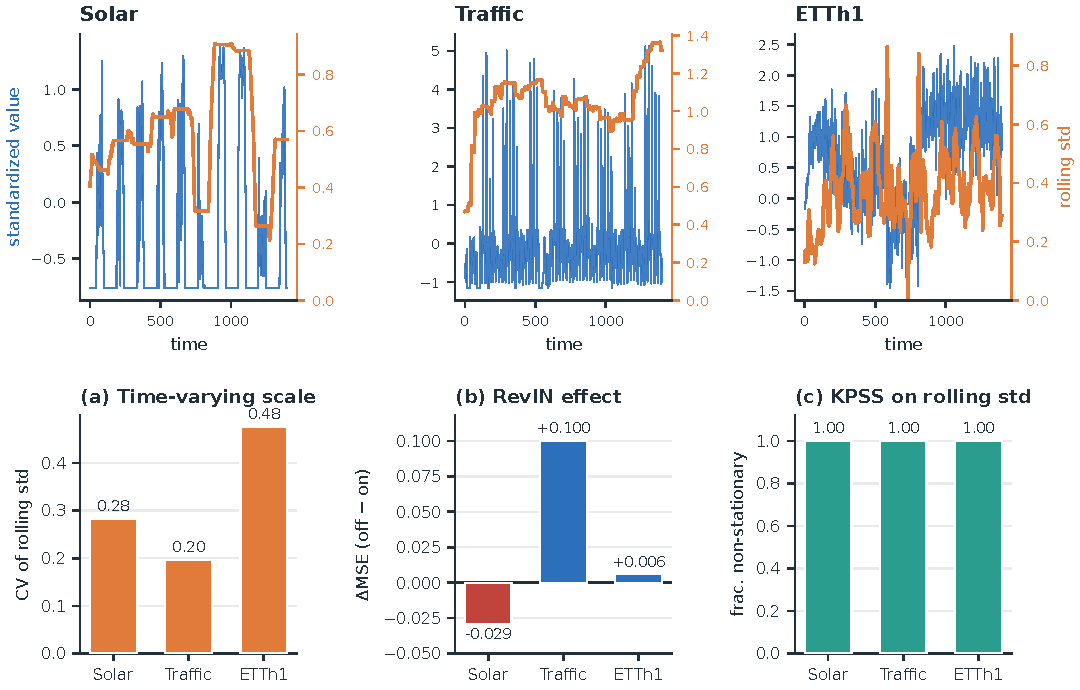
\includegraphics[width=0.92\textwidth]{fig_dispersion.pdf}
\caption{Training-free dispersion diagnostics. \emph{Top:} a
representative standardized channel (blue) with its rolling standard
deviation (orange) for Solar, Traffic, and ETTh1. \textbf{(a)}~Coefficient
of variation of the rolling std. \textbf{(b)}~Measured RevIN effect
($\Delta$MSE, off$-$on): normalizing by the input scale helps Traffic but
hurts Solar. \textbf{(c)}~Fraction of sampled channels whose rolling-std
series a KPSS test declares non-stationary.}
\label{fig:dispersion}
\end{figure}

\subsection{Threats to validity}
Several threats remain, each with the experiment that would resolve it.

\paragraph{Quoted baselines (partly resolved).} Six datasets now have a
unified, five-seed, same-pipeline comparison against seven baselines
(Table~\ref{tab:unified}), which carries the paper's confirmatory accuracy
claims. Three datasets (Solar, Traffic, Exchange) are still quoted from
\cite{smamba} and should be read as indicative only until they are rerun.
Two caveats remain even for the unified table: the repo-native S-Mamba and
ms-Mamba are faithful reimplementations, not the authors' code, and TF4TF
\cite{tf4tf} is not yet included (no public reference implementation);
dropping in official code through the provided adapter would further harden
the comparison.

\paragraph{Statistical power and multiplicity.} With $n{=}3$ seeds, tests
have limited power, and although we apply Benjamini--Hochberg correction,
all 29 component-placement effects fall to $q\ge0.11$: those results are
exploratory. Raising to five and preferably ten seeds, and reporting raw
$p$- and corrected $q$-values for every comparison (as we do in
\texttt{stats\_correction.json}), is needed to move the placement effects
from directional to confirmatory.

\paragraph{Model-selection bias.} This is the most consequential threat.
Although checkpoints are chosen on validation loss, some \emph{switch}
settings --- most visibly disabling RevIN for Solar --- were decided after
inspecting test-set ablations and then folded into the reported
configuration. This is not training-data leakage, but it is selection on the
test signal, and it can inflate the reported numbers for the affected
datasets. The clean protocol, which we recommend for the revision, fixes a
candidate configuration space in advance, selects \emph{every} switch
(normalization, mixer, spectral map, encoder type) on validation data only,
freezes the choice before touching the test set, and reports three clearly
labeled models: a single \emph{fixed} configuration applied everywhere, a
\emph{validation-selected} model, and a \emph{test-oracle} upper bound.
Adding untouched confirmatory datasets (e.g., PEMS03/04/07/08) or previously
unused temporal test blocks would then verify that the validation-only
selection logic generalizes rather than having been fit to the existing nine
benchmarks.

\paragraph{Coverage and efficiency.} Electricity, Traffic, and Exchange
enter the branch matrix at $H{=}96$ only, and the other component ablations
cover only $H{=}96$; schedule sensitivity and head-norm dynamics are not
measured; and the complexity table lacks wall-clock, matched-baseline
throughput, latency, and peak-memory figures. The fixed 96-step look-back
leaves the Traffic weekly-cycle hypothesis untested, while Exchange at
$H{=}720$ remains a notable failure case. Explicit forecasting of
time-varying dispersion is left as future work rather than claimed as part
of the evaluated model.

\section{Conclusion}
\label{sec:conclusion}

\model{} is a forecast-decomposable framework built on state-space
branches --- a DLinear-style temporal backbone, a selective-state-space
correction, an optional frequency pathway, and a switchable cross-variate
mixer, each an independently removable component --- whose purpose is to
diagnose \emph{when} such
components pay rather than to claim universal superiority. In a unified
same-pipeline comparison (five shared seeds, so differences are paired),
\model{} has the lowest average MSE on five of six re-run datasets and, under
Benjamini--Hochberg correction, significantly beats the best in-pipeline
baseline on four (Electricity, ETTh2, ETTm2, ETTh1); it ties on Weather and
is beaten by PatchTST on ETTm1, and three datasets remain quoted-only. This
is a genuine but bounded accuracy result, not a blanket state-of-the-art
claim. The framework's further value is the multiplicity-controlled diagnosis
it enables. Under Benjamini--Hochberg correction, all 29 component-placement
effects are exploratory at three seeds (directionally consistent but not
confirmed), while the branch matrix confirms 9 of 54 tests: the \emph{time}
branch is robustly necessary on the ETTm datasets, whereas confirmatory
evidence for the \emph{frequency} branch narrows to Solar at $H{=}96$. Zero
initialization is accuracy-neutral and retained only for its interpretable
linear starting point. The honest reading is thus conditional component
effectiveness: a confirmed, dataset-specific frequency benefit on Solar, a
broadly confirmed time branch, and a set of directional placement effects
that a higher-powered study should adjudicate. Completing the remaining
strengthening --- the same-pipeline reruns on the three still-quoted datasets,
validation-only switch selection with a labeled test-oracle bound, more seeds
for the ablations, confirmatory datasets, and matched efficiency
measurements --- is the path from this diagnostic framework to a fully
confirmatory submission.



\section*{CRediT authorship contribution statement}
%% TODO (submission): fill in per-author CRediT roles.
\textbf{First Author:} Conceptualization, Methodology, Software,
Investigation, Writing -- original draft. \textbf{Second Author:}
Supervision, Validation, Writing -- review \& editing.

\section*{Declaration of competing interest}
The authors declare that they have no known competing financial interests
or personal relationships that could have appeared to influence the work
reported in this paper.

\section*{Data availability}
All nine benchmark datasets are publicly available (ETT, Weather, Solar,
Electricity, Traffic, Exchange). An anonymized reproducibility package is
provided \emph{at submission} (not withheld until acceptance): it contains
data-download scripts, exact environment versions and backend information,
per-dataset configuration snapshots, commit identifiers, the ablation and
branch-matrix runners, the multiplicity-correction script and its
per-comparison $p$- and $q$-value outputs, seed-level result files,
training logs, and the table-generation scripts; model checkpoints are
included where size permits.
%% TODO (submission): replace with the anonymized repository URL / DOI.

\section*{Declaration of generative AI in the writing process}
%% TODO (submission): complete or remove per the journal's current policy.
During the preparation of this work the authors used generative AI tools to
assist with language editing and code scaffolding; the authors reviewed and
edited all content and take full responsibility for it.

\section*{Acknowledgements}
%% TODO (submission): funding sources.

\bibliographystyle{elsarticle-num}
\bibliography{refs}

\end{document}
